\lecture[2022-05-20]{Pandas I}
\definecolor{gold}{rgb}{0.76, 0.66, 0.06} 
Tabular data is one of the most common data formats and the primary focus of Data 100. In Data 8, we used the \mintinline{text}{Table} class of the \mintinline{text}{datascience} library. Here in Data 100, we use the \mintinline{text}{DataFrame} class of the \mintinline{text}{Pandas} library.
\begin{figure}[ht]
\begin{minipage}{0.5\textwidth}
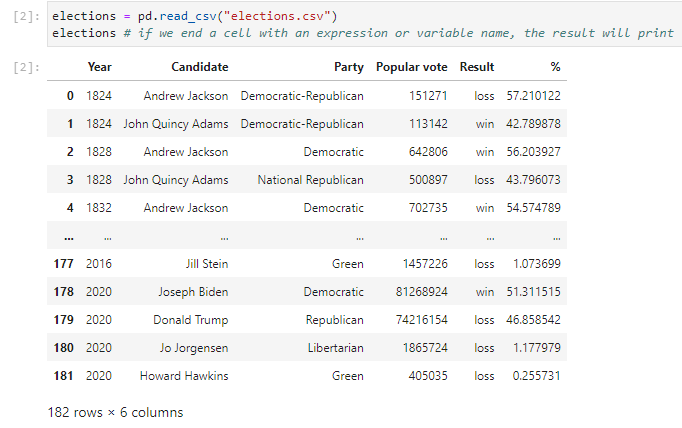
\includegraphics[width=\textwidth]{dataframe.png}\centering
\end{minipage}
\begin{minipage}{0.5\textwidth}
\begin{center}
\includestandalone{figures/3-df}
\end{center}
\end{minipage}
\caption{Left: A sample Pandas DataFrame. Right: A generic DataFrame with a statistical interpretation; rows are samples from the population, columns are features that each sample has.}
\end{figure}
\begin{notebox}[Pandas DataFrame API]
Pandas DataFrame API (application programming interface, or set of applications supported by the class) is very large. When dealing with problems, Google them - they are often found in the documentation or stack overflow.

\href{https://pandas.pydata.org/docs/reference/api/pandas.DataFrame.html}{\color{blue}API Reference}
\end{notebox}

\subsection{Indexing}
One of the most basic tasks of manipulating a DataFrame is to extract rows/columns. Since the Pandas API is very large, this means there are many ways to do things.

Additionally, there is a lot of ``syntactic sugar'' - methods that may be useful and lead to concise code that are not necessary for the library to function (e.g. \mintinline{text}{.head}/\mintinline{text}{.tail}, which select the first/last n rows).

\subsubsection{head/tail}
General Form: \mintinline{text}{df.(head|tail)(<num_rows>)}

Selects the first/last n rows. \mintinline{text}{df.head(5)} is equivalent to \mintinline{text}{df.loc[[0:4]]}, while \mintinline{text}{df.tail(5)} is equivalent to \mintinline{text}{df.loc[[-5:]]}. 

\subsubsection{loc}
General Form: \mintinline{text}{df.loc[<rows>, <cols>]}.

Fundamentally, \mintinline{text}{loc} selects items by label - the bolded text in the top (column names/features) and left (row numbers/samples). Can pass in a list, slice, or single value into \mintinline{text}{loc}.

To select all columns, omit the second argument. To select all rows, pass in \mintinline{text}{:} as the first argument - it is equivalent to selecting the entire array of row numbers.

\begin{figure}[ht]
\begin{minipage}{0.5\textwidth}
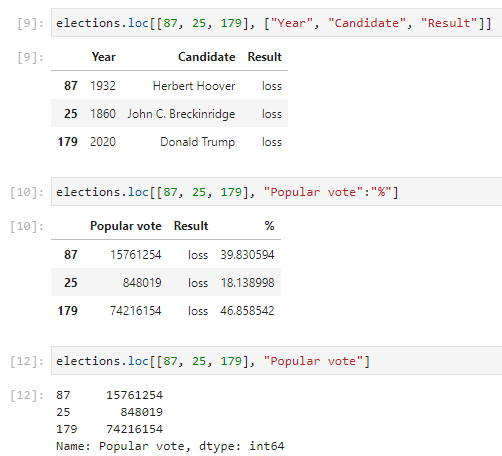
\includegraphics[width=\textwidth]{ex-loc.png}\centering
\end{minipage}
\begin{minipage}{0.5\textwidth}
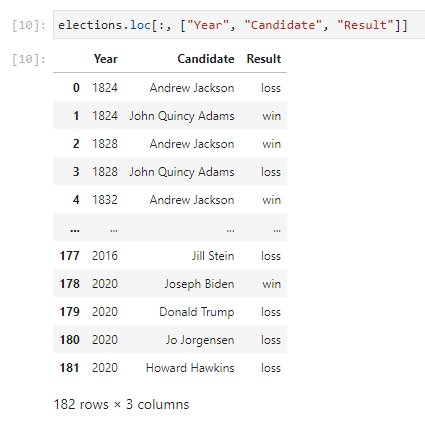
\includegraphics[width=\textwidth]{ex-loc2.png}\centering
\end{minipage}
\caption{Left: selecting different values with \mintinline{text}{loc}. Right: selecting all rows with \mintinline{text}{loc}.}
\end{figure}

\subsubsection{iloc}
General Form: \mintinline{text}{df.iloc[<row-nums>, <col-nums>]}.

Fundamentally, \mintinline{text}{iloc} selects items by number. For rows, this is the same as the label; however, this is not always the case for columns. Like \mintinline{text}{loc}, \mintinline{text}{iloc} can have single values, slices (\mintinline{text}{[<start-num, end-num)}), or arrays passed in as arguments.

And just like \mintinline{text}{loc}, to select all rows, pass in \mintinline{text}{:}, and to select all columns, omit the second argument.

\begin{figure}[ht]
\begin{minipage}{0.5\textwidth}
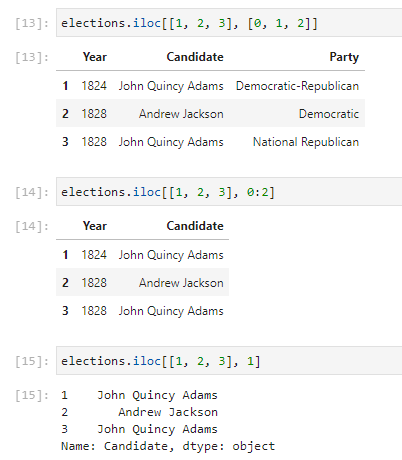
\includegraphics[width=\textwidth]{ex-iloc.png}\centering
\end{minipage}
\begin{minipage}{0.5\textwidth}
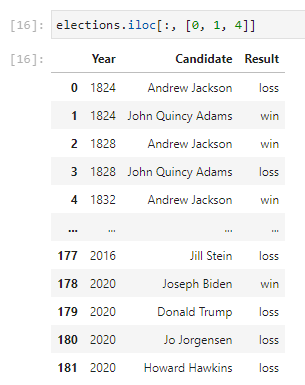
\includegraphics[width=\textwidth]{ex-iloc2.png}\centering
\end{minipage}
\caption{Left: selecting different values with \mintinline{text}{iloc}. Note how instead of column names, we used column numbers. Right: selecting all rows with \mintinline{text}{iloc}.}
\end{figure}

\begin{notebox}[loc vs. iloc]
When deciding between \mintinline{text}{loc} and \mintinline{text}{iloc}, usually \mintinline{text}{loc} is the better choice - it's safer (e.g. will select the right columns if columns are mixed up) and more legible (e.g. \mintinline{text}{["colname1", "colname2"]} over \mintinline{text}{[1, 2]}).

However, \mintinline{text}{iloc} can still be useful - e.g. it would make more sense to index into the middle of a dataframe with \mintinline{text}{iloc}.
\end{notebox}

\subsubsection{[]}
General Form: \mintinline{text}{df[(<row-nums>|col-labels|col-label)]}.

Unlike \mintinline{text}{loc} and \mintinline{text}{iloc}, \mintinline{text}{[]} only takes in one argument rather than rows or columns. The use of \mintinline{text}{[]} changes on the context - i.e., it is context sensitive.
\begin{itemize}
\item For a slice of numbers, it returns the numbered rows.
\item For a list of column names or a single column name, it returns the column(s) in question.
\end{itemize}

\begin{figure}[ht]
\begin{minipage}{0.33\textwidth}
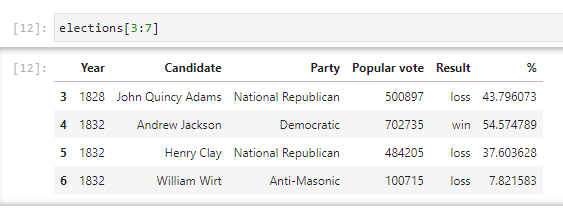
\includegraphics[width=\textwidth]{ex-brac.png}\centering
\end{minipage}
\begin{minipage}{0.34\textwidth}
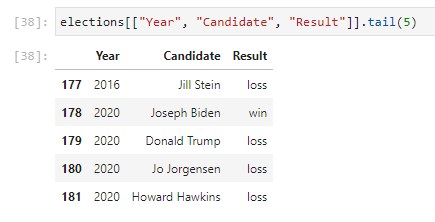
\includegraphics[width=\textwidth]{ex-brac2.png}\centering
\end{minipage}
\begin{minipage}{0.33\textwidth}
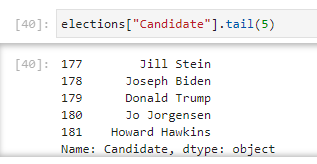
\includegraphics[width=\textwidth]{ex-brac3.png}\centering
\end{minipage}
\caption{\mintinline{text}{[]} in different contexts.}
\end{figure}

\begin{example}[]{Suppose we have the following dataframe \mintinline{text}{weird}:
\begin{center}
\begin{tabular}{@{}crr@{}}
     & \textbf{0} & \textbf{1} \\
\midrule
    \textbf{0} & topdog & topcat \\
    \rowcolor[gray]{0.85}\textbf{1} & botdog & botcat \\
\end{tabular}
\end{center}
What does the following return:
\begin{itemize}
\item \mintinline{text}{weird[1]}
\item \mintinline{text}{weird["1"]}
\item \mintinline{text}{weird[1:]}
\end{itemize}
\tcbline
\begin{itemize}
\item \mintinline{text}{weird[1]}: single column number, so it should return column 1 - i.e. the first column "0".
\begin{center}
\begin{tabular}{@{}cr@{}}
      & \textbf{0} \\
\midrule
    \textbf{0} & topdog \\
    \rowcolor[gray]{0.85} \textbf{1} & botdog \\
\end{tabular}
\end{center}

\item \mintinline{text}{weird["1"]}: single column label, so it should return column "1".
\begin{center}
\begin{tabular}{@{}cr@{}}
      & \textbf{1} \\
\midrule
    \textbf{0} & topcat \\
    \rowcolor[gray]{0.85} \textbf{1} & botcat \\
\end{tabular}
\end{center}

\item \mintinline{text}{weird[1:]}: row slices, so just the first row and beyond.
\begin{center}
\begin{tabular}{@{}crr@{}}
     & \textbf{0} & \textbf{1} \\
\midrule
    \textbf{1} & botdog & botcat \\
\end{tabular}
\end{center}

\end{itemize}
}
\end{example}
\begin{notebox}[\normalfont \mintinline{text}{[]} \textbf{Usage and Dot Notation}]
Whereas \mintinline{text}{loc} and \mintinline{text}{iloc} both accept multiple arguments, \mintinline{text}{[]} does not and selects based on context. Therefore, the syntax is more precise and preferred for real world practice compared to \mintinline{text}{loc}.

Another way to index is with dot notation; more info can be found \href{https://www.dataschool.io/pandas-dot-notation-vs-brackets/}{\color{blue}here}.
\end{notebox}

\subsection{DataFrames, Series, and Indices}
Notice in the previous examples above, if we select only a single column, the notebook returns a different format. This is since the return output is a Series and not a DataFrame.

\begin{minted}{python}
type(elections) # DataFrame
type(elections["Candidate"]) # Series
\end{minted}

This leads into the Pandas data structures. Here are the three fundamental data structures in Pandas:
\begin{itemize}
\item \textbf{DataFrame}: 2D Tabular Data.
\item \textbf{Series}: 1D single-column/columnar data.
\item \textbf{Index}: sequence of row labels.
\end{itemize}
We can think of a dataframe as a collection of series that all have the same index.

Indices are not necessarily row numbers; they can also be non-numeric and have names, e.g. State. They also do not have to be unique.

However, column names are almost always unique. (e.g. it would not make sense to have two columns with the same name, but you can force duplicate columns to have them have the same column name).

If you want row/column labels: you can use \mintinline{text}{df.index} for row labels and \mintinline{text}{df.columns} for column labels.
\begin{notebox}[Getting a DataFrame instead of a Series]
If you want a DataFrame instead of a Series input, there are two ways to do so:
\begin{itemize}
\item \mintinline{text}{Series.toFrame()} method.
\item Enclose the single column of interest in a list (e.g. \mintinline{text}{df[[<col-name>]]} as opposed to \mintinline{text}{df[col-name]})
\end{itemize}
\end{notebox}

\subsection{Conditional Selection}
\mintinline{text}{loc} also supports Boolean array input (usually generated by using logical operators on Series). This can be combined with operators, allowing for filtering with multiple criteria
\begin{minted}{python}
elections[elections["Party"] == "Independent"] # checks the Party series for each entry, keeps the entries which the party is independent

elections[(elections["Result"] == "win") & (elections["%"] < 47)] # checks if the election result is a win and if the winning percent is less than 47%
\end{minted}
\begin{example}[]{Which of the following statements returns a DataFrame of the first 3 candidate names only for candidates that won more than 50\% of the vote?
\tcbline
Using \mintinline{text}{loc}: select all the candidates (rows) that have an election percent > 50, choose candidate, year columns, first three rows that satisfy the condition (head).

End Code: \mintinline{text}{elections.loc[[elections['%'] > 50, ["Candidate", "Year"]].head(3)}
}

Using \mintinline{text}{iloc}: The columns in question are candidate (0) and Year (3), and the first three rows that satisfy the conditions are 0, 3, 5. Therefore, the end code should be \mintinline{text}{elections.iloc[[0, 3, 5], [0, 3]]}.
\end{example}

While boolaen array selection is useful, it can lead to overly verbose code when there are complex selections. There are many alternative functions to make the code more concise:
\begin{itemize}
\item \mintinline{text}{.isin}: returns True if the row value is in an array of results.
\item \mintinline{text}{.str.startswith}: return True if the row value starts with the string provided.
\item \mintinline{text}{.query}: Similar to SQL queries select keyword (select rows which fit the criteria). can access Python variables with \mintinline{text}{@<var-name>}.
\item \mintinline{text}{.groupby.filter}: to be discussed in the next lecture.
\end{itemize}

\begin{minted}{python}
# original, verbose code
elections[(elections["Party"] == "Anti-Masonic")  | 
          (elections["Party"] == "American")      |
          (elections["Party"] == "Anti-Monopoly") |
          (elections["Party"] == "American Independent")]

# .isin
a_parties = ["Anti-Masonic", "American", "Anti-Monopoly", "American Independent"]
elections[elections["Party"].isin(a_parties)]
# .str.startswith
elections[elections["Party"].str.startswith("A")]
# query - select rows of elections after 2000 and the result is a win 
elections.query('Year >= 2000 and Result == "win"')
# query with @
parties = ["Republican", "Democratic"]
elections.query('Result == "win" and Party not in @parties') # select winners that don't belong to republican/democratic parties
\end{minted}

\subsection{Utility Functions}
Pandas Series/DataFrames support mathematical, NumPy, and built-in functions as long as the data is numerical. Additionally, Pandas has its own utility functions:
\begin{itemize}
\item \mintinline{text}{size/shape}: size returns the amount of data entries (rows by columns), while shape returns the shape (rows, columns).
\item \mintinline{text}{describe}: gives a brief description of the numerical data, returning the count, mean/stdev, and 5 points (min, 25\%, 50\%, 75\%, and max).
\item \mintinline{text}{sample}: samples a random selection of rows without replacement (add \mintinline{text}{replace=True}) for replacement. Can be chained with other methods and operators (e.g. \mintinline{text}{query}, \mintinline{text}{iloc}, etc.).
\item \mintinline{text}{Series.value_counts}: counts the number of occurences of each unique value (returned as a series of value-count).
\item \mintinline{text}{Series.unique}: returns an array of all unique values in a Series.
\item \mintinline{text}{sort_values}: sorts values in a Series or a DataFrame (must list column on which to sort for a DataFrame) in ascending order (for descending order, set \mintinline{text}{ascending=False}).
\end{itemize}

